%%%%%%%%%%%%%%%%%%%%%%%%%
\section{ACAS XU}
%%%%%%%%%%%%%%%%%%%%%%%%%

\begin{figure}[t]
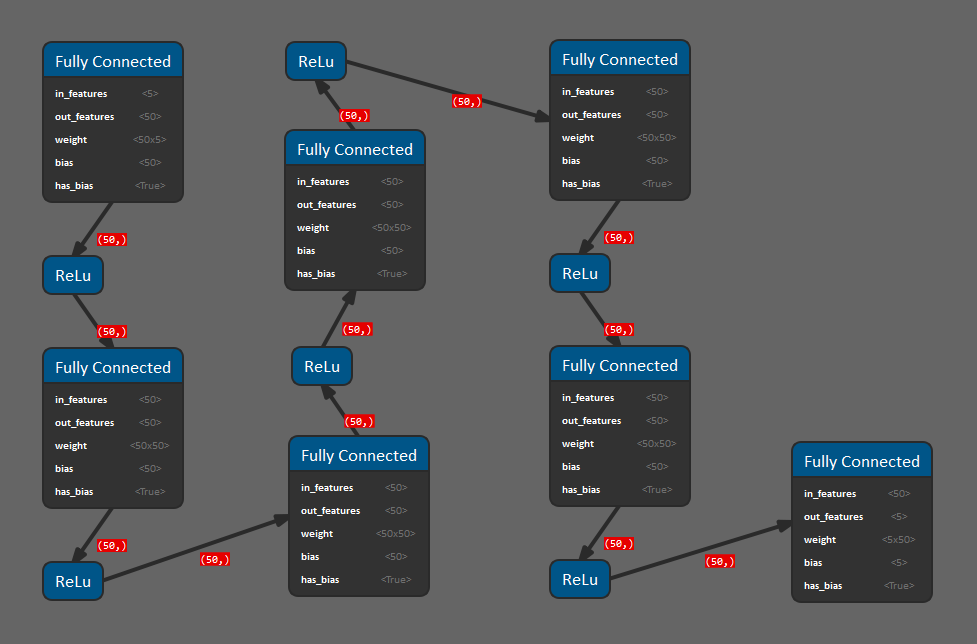
\includegraphics[width=1\textwidth]{imgs/ACAS_CCNN.png}
\label{img:acas-architecture}
\caption{Graphical representation of a ONNX model of an ACAS XU network. 
	The image is generated in \href{https://github.com/NeVerTools/NeVer2}
	{NeVer2}.}
\end{figure}

We consider a standard example of an ACAS XU network with 6 hidden
layers of 50 ReLU neurons each; the input and output layers consist 
of 5 neurons. In Figure~\ref{img:acas-architecture} we show a graphical
representation of this model. The ACAS XU network acts as a function 
$\nu : I^5 \to O^5$ with $I = O = \mathbb{R}$.  A property of interest 
for this kind of network can be stated as follows: 

\begin{equation}
\label{eq:acas-property1}
\begin{array}{l}
- \varepsilon_0 \leq x_0 \leq \varepsilon_0 \\
- \varepsilon_1 \leq x_1 \leq \varepsilon_1 \\
- \varepsilon_2 \leq x_2 \leq \varepsilon_2 \\
- \varepsilon_3 \leq x_3 \leq \varepsilon_3 \\
- \varepsilon_4 \leq x_4 \leq \varepsilon_4 \\
y_0 - y_1 \leq 0 \\
y_0 - y_2 \leq 0 \\
y_0 - y_3 \leq 0 \\
y_0 - y_4 \leq 0 \\
\end{array}
\end{equation}

where $\varepsilon_i \in \mathbb{R}+$ with $0 \leq i \leq 4$ are
arbitrary positive input noise constants, $(x_0, \ldots, x_4) 
\in \mathbb{R}^5$ is a sample of the input vector and 
$(y_0, \ldots, y_4) \in \mathbb{R}^5$ is the corresponding output
vector $(y_0, \ldots, y_4) = \nu((x_0, \ldots, x_4))$.

The property can be experessed in the SMT-LIB language using
specific identifiers for input and output vectors derived from
the identifiers used in the ONNX model. In particular, ONNX only
provides an identifier for the output of each layer and a global 
identifier for the network input; for this reason we identify the 
input tensor as $\mathbf{X}$ and the output tensor as the last 
Fully Connected (\textit{Gemm}) node identifier $\mathbf{FC6}$, 
both with dimension 5. We can then express property 
(\ref{eq:acas-property1}) in SMTLIB as:
\begin{lstlisting}
	
; definition of the variables of interest
(declare-fun X_0 () Real)
(declare-fun X_1 () Real)
(declare-fun X_2 () Real)
(declare-fun X_3 () Real)
(declare-fun X_4 () Real)

(declare-fun FC6_0 () Real)
(declare-fun FC6_1 () Real)
(declare-fun FC6_2 () Real)
(declare-fun FC6_3 () Real)
(declare-fun FC6_4 () Real)

; definition of the constraints
(assert (<= X_0 eps_0))
(assert (>= X_0 -eps_0))
(assert (<= X_1 eps_1))
(assert (>= X_1 -eps_1))
(assert (<= X_2 eps_2))
(assert (>= X_2 -eps_2))
(assert (<= X_3 eps_3))
(assert (>= X_3 -eps_3))
(assert (<= X_4 eps_4))
(assert (>= X_4 -eps_4))

(assert (<= (- FC6_0 FC6_1) 0.0))
(assert (<= (- FC6_0 FC6_2) 0.0))
(assert (<= (- FC6_0 FC6_3) 0.0))
(assert (<= (- FC6_0 FC6_4) 0.0))
\end{lstlisting}
This fragment of code is compliant with the SMT-LIB 2 language standard
and it defines the property of interest in term of input-output
relations.  Clearly, this code is not complete in terms of internal
constraints of the network: these will be extracted based on the
verification methodology of interest from the ONNX model of the network.

%%%%%%%%%%%%%%%%%%%%%%%%%
\section{MNIST}
%%%%%%%%%%%%%%%%%%%%%%%%%

\begin{figure}[t]
	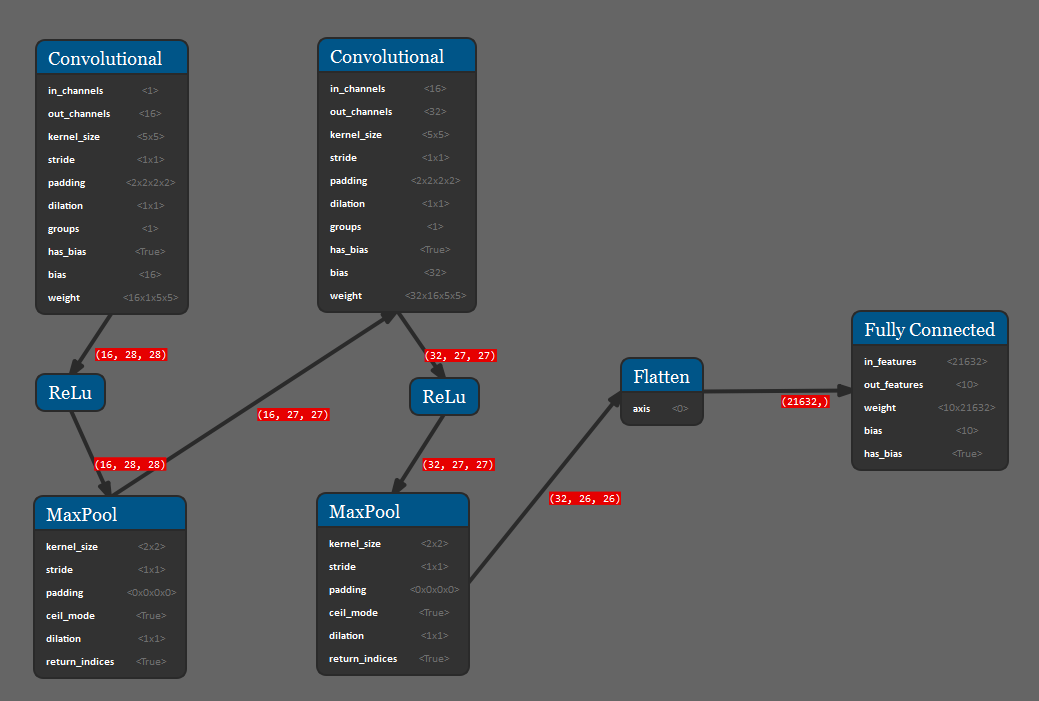
\includegraphics[width=1\textwidth]{imgs/MNIST_conv_CCNN.png}
	\label{img:mnist-architecture}
	\caption{Graphical representation of a ONNX model of a convolutional
		MNIST network. The image is generated in 
		\href{https://github.com/NeVerTools/NeVer2}{NeVer2}.}
\end{figure}

We consider a standard example of a convolutional MNIST network with 
two convolutional layers consisting of a convolution with a 5 $\times$ 5
kernel with 2 pixel padding, a ReLU activation function and a Max Pooling
with a 2 $\times$ 2 kernel. The first convolution generates 16 channels,
and the second 32; the result is flattened to a single vector which is
finally fed to a Fully Connected layer. The input layer consists of a 
three-dimensional tensor $1 \times 28 \times 28$ and the output layer 
consists of 10 neurons for the classification. 
In Figure~\ref{img:mnist-architecture} we show a graphical
representation of this model. A network for classifying objects in the MNIST
dataset is a function $\nu : I^{1,28,28} \to O^{10}$ with $I = O = \mathbb{R}$.

A local robustness property can be expressed in a similar way with respect
to the ACAS XU network: for a local sample $\hat{x}$ such that 
$\nu(\hat{x}) = y_9$ and an input noise $\varepsilon$, the classification 
should not change for a $\varepsilon$ perturbation.

\begin{equation}
	\label{eq:mnist-property1}
	\begin{array}{l}
		\forall i \in [0, 783] : 
			\hat{x} - \varepsilon \leq x_i \leq \hat{x} + \varepsilon \\	
		\forall j \in [0, 8] : y_j - y_9 \leq 0
	\end{array}
\end{equation}

In order to represent correctly the variables corresponding to multi-dimensional
tensors we allow two different notations: one that distinguishes the 
single dimensions and one that flattens the tensor in a single 1-D array.

\paragraph{Tensor representation.}
Let $x^D$ be a tensor in a $D$-dimensional space. We associate the dimensional
subscripting with a single underscore for separating the variable name and the
variable subscript, and $D-1$ dashes for separating the dimension values:
\begin{itemize}
	\item \textit{1-D} tensor: X\_0, X\_1, \ldots, X\_n
	\item \textit{2-D} tensor: X\_0-0, X\_0-1, \ldots, X\_1-0, X\_1-1, \ldots, X\_n-m
	\item \textit{3-D} tensor: X\_0-0-0, \ldots, X\_i-j-k, \ldots, X\_n-m-p
	\item $\cdots$
\end{itemize}
In the example above, X\_0-3-2 corresponds to the input $x_{0,3,2} \in x^3$ in 
tensor form.
\myremark{Please note that this notation is encouraged, as it provides a clearer
interpretation of the property.}

\paragraph{Array representation.}
Let $x^D$ be a tensor in a $D$-dimensional space. We provide the following
algorithm to flatten it in a single 1-$D$ array.
\begin{algorithm}
	\caption{Tensor flattening}
	\label{alg:flatten}
	\begin{algorithmic}[1]
		\Procedure{flatten}{$x$}
			\State $idx = 0$
			\For{$a == 0$ to $N_1$}
				\For{$b == 0$ to $N_2$}
					\State $\ldots$
					\For{$k == 0$ to $N_k$}
						\State X\_$idx$ = $x_{a, b, \ldots, k}$
						\State $idx = idx + 1$
					\EndFor
				\EndFor
			\EndFor
		\EndProcedure
	\end{algorithmic}
\end{algorithm}

All properties which comply with either representation should be accepted
and readable. An example in the SMT-LIB language is provided as follows,
highlighting the two possibilities for defining the variables.

\begin{lstlisting}
	
; definition of the variables of interest
(declare-fun X_0 () Real) ; (declare-fun X_0-0-0 () Real)
(declare-fun X_1 () Real)
(declare-fun X_2 () Real)
...
(declare-fun X_782 () Real) ; (declare-fun X_0-26-27 () Real)
(declare-fun X_783 () Real) ; (declare-fun X_0-27-27 () Real)

(declare-fun FC0_0 () Real)
(declare-fun FC0_1 () Real)
(declare-fun FC0_2 () Real)
...
(declare-fun FC0_9 () Real)

; definition of the constraints
(assert (<= X_0 eps)) ; (assert (<= X_0-0-0 eps))
(assert (>= X_0 -eps)) ; (assert (>= X_0-0-0 -eps))
...
(assert (<= X_783 eps)) ; (assert (<= X_0-27-27 eps))
(assert (>= X_783 -eps)) ; (assert (>= X_0-27-27 -eps))

(assert (<= (- FC0_0 FC0_9) 0.0))
(assert (<= (- FC0_1 FC0_9) 0.0))
...
(assert (<= (- FC0_8 FC0_9) 0.0))
\end{lstlisting}